% compile using: agda --latex; result will then be in the latex/ subfolder
\documentclass[11pt,utf8,notheorems,compress,t,aspectratio=169]{beamer}
\usepackage{etex}

\usepackage{pgfpages}
\usepackage[export]{adjustbox}

% Workaround for the issue described at
% https://tex.stackexchange.com/questions/164406/beamer-using-href-in-notes.
\newcommand{\fixedhref}[2]{\parbox[t][0pt][t]{0pt}{\vspace*{-\paperheight}\vspace*{-0.6em}\href{#1}{#2}}\href{#1}{#2}}

\usepackage[english]{babel}

\usepackage{mathtools}
\usepackage{xspace}
\usepackage{booktabs}
\usepackage{stmaryrd}
\usepackage{amssymb}
\usepackage{manfnt}
\usepackage{array}
\usepackage{ragged2e}
\usepackage{multicol}
\usepackage{tabto}
\usepackage{xstring}
\usepackage{proof}
\usepackage{agda}
\usepackage[all]{xy}
\xyoption{rotate}
\usepackage{tikz}
\usetikzlibrary{calc,shapes,shapes.callouts,shapes.arrows,patterns,fit,backgrounds,decorations.pathmorphing,positioning,svg.path}
\hypersetup{colorlinks=true}
\usepackage[dvipsnames]{xcolor}
\usepackage{fontawesome5}

\DeclareFontFamily{U}{bbm}{}
\DeclareFontShape{U}{bbm}{m}{n}
   {  <5> <6> <7> <8> <9> <10> <12> gen * bbm
      <10.95> bbm10%
      <14.4>  bbm12%
      <17.28><20.74><24.88> bbm17}{}
\DeclareFontShape{U}{bbm}{m}{sl}
   {  <5> <6> <7> bbmsl8%
      <8> <9> <10> <12> gen * bbmsl
      <10.95> bbmsl10%
      <14.4> <17.28> <20.74> <24.88> bbmsl12}{}
\DeclareFontShape{U}{bbm}{bx}{n}
   {  <5> <6> <7> <8> <9> <10> <12> gen * bbmbx
      <10.95> bbmbx10%
      <14.4> <17.28> <20.74> <24.88> bbmbx12}{}
\DeclareFontShape{U}{bbm}{bx}{sl}
   {  <5> <6> <7> <8> <9> <10> <10.95> <12> <14.4> <17.28>%
      <20.74> <24.88> bbmbxsl10}{}
\DeclareFontShape{U}{bbm}{b}{n}
   {  <5> <6> <7> <8> <9> <10> <10.95> <12> <14.4> <17.28>%
      <20.74> <24.88> bbmb10}{}
\DeclareMathAlphabet{\mathbbm}{U}{bbm}{m}{n}
\SetMathAlphabet\mathbbm{bold}{U}{bbm}{bx}{n}

\usepackage{pifont}
\newcommand{\cmark}{\ding{51}}
\newcommand{\xmark}{\ding{55}}
\DeclareSymbolFont{extraup}{U}{zavm}{m}{n}
\DeclareMathSymbol{\varheart}{\mathalpha}{extraup}{86}

\graphicspath{{images/}}

\usepackage[protrusion=true,expansion=true]{microtype}

\setlength\parskip{\medskipamount}
\setlength\parindent{0pt}

\title{Towards topological type theory for decrypting transfinite methods in classical mathematics}

\author{Ingo Blechschmidt}
\date{June 9th, 2025}

%\setbeameroption{show notes on second screen=bottom}
\newcommand{\jnote}[2]{\only<#1>{\note{\setlength\parskip{\medskipamount}\footnotesize\justifying#2\par}}}
\makeatletter
\setbeamertemplate{note page}
{%
  {%
    \scriptsize
    \insertvrule{.25\paperheight}{white!90!black}
    \vskip-.25\paperheight
    \nointerlineskip
    \vbox{
      %\hfill\insertslideintonotes{0.25}\hskip-\Gm@rmargin\hskip0pt%
      %\vskip-0.25\paperheight%
      %\nointerlineskip
      \begin{pgfpicture}{0cm}{0cm}{0cm}{0cm}
        \begin{pgflowlevelscope}{\pgftransformrotate{90}}
          {\pgftransformshift{\pgfpoint{-2cm}{0.2cm}}%
          \pgftext[base,left]{\footnotesize\the\year-\ifnum\month<10\relax0\fi\the\month-\ifnum\day<10\relax0\fi\the\day}}
        \end{pgflowlevelscope}
      \end{pgfpicture}}
    \nointerlineskip
    \vbox to .25\paperheight{\vskip0.5em
      \hbox{\insertshorttitle[width=8cm]}%
      \setbox\beamer@tempbox=\hbox{\insertsection}%
      \hbox{\ifdim\wd\beamer@tempbox>1pt{\hskip4pt\raise3pt\hbox{\vrule
            width0.4pt height7pt\vrule width 9pt
            height0.4pt}}\hskip1pt\hbox{\begin{minipage}[t]{7.5cm}\def\breakhere{}\insertsection\end{minipage}}\fi%
      }%
      \setbox\beamer@tempbox=\hbox{\insertsubsection}%
      \hbox{\ifdim\wd\beamer@tempbox>1pt{\hskip17.4pt\raise3pt\hbox{\vrule
            width0.4pt height7pt\vrule width 9pt
            height0.4pt}}\hskip1pt\hbox{\begin{minipage}[t]{7.5cm}\def\breakhere{}\insertsubsection\end{minipage}}\fi%
      }%
      \setbox\beamer@tempbox=\hbox{\insertshortframetitle}%
      \hbox{\ifdim\wd\beamer@tempbox>1pt{\hskip30.8pt\raise3pt\hbox{\vrule
            width0.4pt height7pt\vrule width 9pt
            height0.4pt}}\hskip1pt\hbox{\insertshortframetitle[width=7cm]}\fi%
      }%
      \vfil}%
  }%
  \vskip.25em
  \nointerlineskip
  \insertnote
}
\makeatother

%\useinnertheme[shadow=true]
\setbeamerfont{block title}{size={}}

\useinnertheme{rectangles}

\usecolortheme{orchid}
\usecolortheme{seahorse}
\definecolor{mypurple}{RGB}{253,73,34}
\definecolor{mypurpledark}{RGB}{100,0,150}
\setbeamercolor{structure}{fg=mypurple}
\setbeamercolor*{title}{bg=mypurple,fg=white}
\setbeamercolor*{titlelike}{bg=mypurple,fg=white}
\setbeamercolor{frame}{bg=black}

\usefonttheme{serif}
\usepackage[T1]{fontenc}
\usepackage{libertine}

% lifted from https://arxiv.org/abs/1506.08870
\DeclareFontFamily{U}{min}{}
\DeclareFontShape{U}{min}{m}{n}{<-> udmj30}{}
\newcommand\yon{\!\text{\usefont{U}{min}{m}{n}\symbol{'210}}\!}

\newcommand{\A}{\mathcal{A}}
\newcommand{\B}{\mathcal{B}}
\newcommand{\C}{\mathcal{C}}
\newcommand{\M}{\mathcal{M}}
\renewcommand{\AA}{\mathbb{A}}
\newcommand{\BB}{\mathbb{B}}
\newcommand{\pp}{\mathbbm{p}}
\newcommand{\MM}{\mathbb{M}}
\newcommand{\E}{\mathcal{E}}
\newcommand{\F}{\mathcal{F}}
\newcommand{\FF}{\mathbb{F}}
\newcommand{\G}{\mathcal{G}}
\newcommand{\J}{\mathcal{J}}
\newcommand{\GG}{\mathbb{G}}
\renewcommand{\O}{\mathcal{O}}
\newcommand{\K}{\mathcal{K}}
\newcommand{\NN}{\mathbb{N}}
\newcommand{\QQ}{\mathbb{Q}}
\newcommand{\RR}{\mathbb{R}}
\newcommand{\TT}{\mathbb{T}}
\newcommand{\PP}{\mathbb{P}}
\newcommand{\ZZ}{\mathbb{Z}}
\newcommand{\CC}{\mathbb{C}}
\renewcommand{\P}{\mathcal{P}}
\newcommand{\aaa}{\mathfrak{a}}
\newcommand{\bbb}{\mathfrak{b}}
\newcommand{\ccc}{\mathfrak{c}}
\newcommand{\ppp}{\mathfrak{p}}
\newcommand{\fff}{\mathfrak{f}}
\newcommand{\mmm}{\mathfrak{m}}
\newcommand{\defeq}{\vcentcolon=}
\newcommand{\defeqv}{\vcentcolon\equiv}
\newcommand{\Cov}{\mathrm{Cov}}
\renewcommand{\_}{\mathpunct{.}}
\newcommand{\?}{\,{:}\,}
\newcommand{\speak}[1]{\ulcorner\text{\textnormal{#1}}\urcorner}
\newcommand{\inv}{inv.\@}
\newcommand{\forces}{\vDash}
\newcommand{\ind}{\ensuremath{_\text{ind}}\xspace}
\newcommand{\sinf}{\ensuremath{_\infty}}
\newcommand{\impl}{\ensuremath{_\text{impl}}\xspace}
\newcommand{\formalized}{{\color{NavyBlue!75!White}{\raisebox{-0.5pt}{\scalebox{0.8}{\faCog}}}}}

\setbeamertemplate{blocks}[shadow=false]

\newenvironment{indentblock}{%
  \list{}{\leftmargin\leftmargin}%
  \item\relax
}{%
  \endlist
}

% Adapted from https://latex.org/forum/viewtopic.php?t=2251 (Stefan Kottwitz)
\newenvironment<>{hilblock}{
  \begin{center}
    \begin{minipage}{9.05cm}
      \setlength{\textwidth}{9.05cm}
      \begin{actionenv}#1
        \def\insertblocktitle{}
        \par
        \usebeamertemplate{block begin}}{
        \par
        \usebeamertemplate{block end}
      \end{actionenv}
    \end{minipage}
  \end{center}}

\newenvironment{changemargin}[2]{%
  \begin{list}{}{%
    \setlength{\topsep}{0pt}%
    \setlength{\leftmargin}{#1}%
    \setlength{\rightmargin}{#2}%
    \setlength{\listparindent}{\parindent}%
    \setlength{\itemindent}{\parindent}%
    \setlength{\parsep}{\parskip}%
  }%
  \item[]}{\end{list}}

\tikzset{
  invisible/.style={opacity=0,text opacity=0},
  visible on/.style={alt={#1{}{invisible}}},
  alt/.code args={<#1>#2#3}{%
    \alt<#1>{\pgfkeysalso{#2}}{\pgfkeysalso{#3}}}
}

% https://tex.stackexchange.com/questions/172336/drawing-roman-laurel-leaves-spqr-in-tikz
\tikzset{
  laurel-wreath/.pic = {
    \fill svg{M14.4-24.6c-1.5-1.5-2.6-3.3-3.1-5.3l-.4-1.7c-.2-1.1-.2-4.1 .2-5.7 .2-.9 .3-1.3 .5-1.3l1.4 1.1 2.5 2.4c2.7 2.5 5.2 6 5.8 8 .2 .6-.5 .3-2.2-.9-1.6-1.3-3.3-2.6-5-3.8l.1 1.4c.2 1.4 .5 2.7 1.1 4.6s.8 2.5 .5 2.5l-1.4-1.3zm69.6 1.1 .3-1.2c.8-2.3 1.3-4.8 1.6-7.3l-1.5 1.1c-1.3 .9-2.6 1.9-3.7 3-1.6 1.1-2 1.3-2.1 1 .7-1.8 1.6-3.4 2.8-4.9 1.3-1.7 6.5-6.8 7-6.8 .2 0 .3 .2 .3 .5l.3 1.6c.3 2.2 .2 5.7-.5 7.4-.8 1.9-1.6 3.1-3 4.7-1.1 1.1-1.4 1.3-1.5 .9z};
    \fill svg{M10-29.4c-.8-1.1-1.4-2.2-2-4.1l-.7-3.5c-.2-3 .2-4.4 1.4-8.3l.5-1.4c.2-1.3 .3-1.9 .6-1.9 .3-.2 .6 .3 .7 .8s.9 2.2 1.9 3.6c1.4 2.2 2.7 4.4 3.9 6.6l.9 2.7c0 .6 0 .6-.3 .6-.6 0-4.9-4.4-5.8-6l-.2-.6-.1 1.7-.3 2.8c-.3 2.7-.3 3.8 0 5.5 .6 2 .5 2.4-.5 1.5zm79.2 .3 .4-2.4c.2-1.3 .2-2.7-.1-4.9l-.3-2.8v-1.6l-.7 1c-.8 1.3-5 5.5-5.5 5.5s-.5-.3 .2-1.9c.5-1.7 1.4-3.3 3.3-6.5 2.4-3.6 2.7-3.9 2.8-4.7 .5-1.3 .5-1.4 .8-1.2 .3 0 .6 .8 .6 1.5l.7 2.4c.9 2.7 1.1 3.6 1.2 6 .2 3.1-.5 6-2 8.2-.8 1.3-1.3 1.7-1.4 1.5z};
    \fill svg{M5-40c-.4-3.2-.1-6.5 .9-9.6 .5-1.1 1.6-2.8 2.2-3.4l1.3-1.6 2-2.7 .2 .6c.1 1.3 .4 2.6 .9 3.8l.3 1c.8 1.7 1.1 2.7 1.6 5.3 .6 2.5 .6 4.6 .2 4.6-.3 0-.9-.8-1-1.1l-.5-.8c-1.4-2-3-5.2-2.9-6.5-.9 2.7-2 5.4-3.5 7.9l-.3 .8-.3 .8c0 .5-.6 1.6-.8 1.6l-.3-.7zm89.2 .2-.2-.5-.3-.9-1.1-2.7-1.1-2.4c-.6-1.4-1.2-2.8-1.6-4.2l-.3 .9c-.3 1.3-1.6 3.9-3 6-1.3 2-1.6 2-1.5 0s1.1-6.3 2.2-9c.8-1.7 1.1-3.1 .9-4.1-.2-1.1 .5-.8 2.2 1.8 3.3 4.4 3.8 5.4 4.4 7.8 .6 2.4 .5 7.7-.3 7.8l-.3-.5z};
    \fill svg{M13.9-50.1c-.5-1.9-.8-3.9-.9-5.8-.2-1.6-.1-3.3 .1-4.9-.3 .8-1.7 2.5-4.2 5.1l-3 4.9-.3 .1c-.3 0-.3-2.2 0-3.3 .8-3 1.4-4.6 2.5-6.1 .9-1.3 1.7-1.9 2.5-2.5 1.1-.6 2.7-1.9 3.5-2.7 .9-.9 1.9-1.4 2.2-1.4v1.1l-.3 6.6c0 6.8 .2 6.3-1 8.9-.5 1.1-.8 1.1-1.1 0zm70.8-.4c-.8-2.2-.8-2.5-.7-6.3-.1-2.7-.1-5.5-.2-8.2-.3-1.6-.3-1.9 .5-1.6l.6 .5c1.4 1.4 3 2.5 3.9 3.1 1.3 .9 1.9 1.6 2.7 2.6l.6 .7 .2 .4 .2 .3c.8 .9 2 4.9 2 6.9 .2 1.9-.2 1.9-.9 .5-.7-1.4-1.5-2.7-2.6-4-1.6-1.5-3-3.2-4.2-5 .4 3 .3 6-.5 9 0 .8-.5 2.2-.8 2.3-.2 0-.5-.3-.8-1.2z};
    \fill svg{M16.4-58.5l.2-1.5 .3-3.7c.2-2.8 .3-3.5 1.1-5.4l.7-1.3-.5 .4-1 .7c-.5 .4-1.1 .8-1.5 1.3l-.5 .3-1.9 1.6c-2.2 1.6-2.7 2-3.9 3.6-.5 .8-1.1 1.3-1.3 1.3-.5 0 0-2.4 1.1-4.7 1.5-3.4 4.3-6 7.7-7.4l1.3-.4 1.9-.4 2-.5c1.4 0 1.4 0 1 1.1-.5 .8-.8 2-1.1 4.2-.3 2.3-1.1 4.5-2.2 6.5l-.4 .6c-.6 1.1-1.3 2.1-2 3.2-.5 .6-.8 .8-1 .5zm66.3-.2c-.8-.9-2.8-4.4-3.5-6.1-.6-1.3-.9-2.5-1.1-3.5-.2-2.1-.7-4.1-1.5-6 0-.3 0-.3 1.2-.3l2.1 .5 1.9 .4 1.2 .4 .6 .1 1 .6c3 1.4 5.7 4.6 6.8 8.5l.7 2.6c-.2 .6-.5 .5-1.4-.7-2.2-2.7-4.8-5-7.7-6.9l-1.7-1.3 .6 1.3c.3 .6 .6 1.2 .8 1.9l.3 2.5 .3 3.9c.3 2.4 .2 2.8-.6};
    \fill svg{M21.6-66.1l.4-1.1 .9-3.2c.3-1.9 1.1-3.3 2.4-4.7l.4-.8-1.2 .2-2.2 .3c-2.7 .3-5.3 1.2-7.7 2.5-.6 .5-1.3 .6-1.3 .3 0-.5 .9-1.9 2-2.9 .8-.9 2-1.9 3.2-2.6l.9-.4 2.2-1c.3-.2 1.3-.3 3.2-.1 3 0 4.1 .2 6.3 .7l1.1 .4c.5 .2 .6 .6 .3 .6-.5 0-1.4 .9-1.9 1.7l-1.2 1.8c-1.7 2.8-2.2 3.5-4.6 5.9l-3 2.7-.2-.3zm53.9-2c-2.7-2.8-3.5-3.8-5.4-6.8-.9-1.6-1.4-2.4-1.9-2.5l-.8-.5c-.3 0-.2-.5 .4-.6l1.1-.4c1.9-.6 3-.8 5.6-.9l3.3 .2c2 .6 3.8 1.5 5.4 2.8 .3 0 1.9 1.6 2.5 2.4l.9 1.8c0 .3-.3 .2-1.9-.6-2.8-1.4-4.4-1.9-7.7-2.2l-2.2-.5c-.9-.2-.9-.2-.6 .2 .6 .5 1.7 2 2.1 2.8l.9 2.5c.3 1.5 .6 3 .9 4.6l-2.6-2.3z};
    \fill svg{M34.1-78.7c-3.4-1.3-6.9-2.1-10.6-2.5-.9 0-1.4 0-2.3 .3-2 .5-2 0 0-1.3l2.8-1.2c1.4-.5 1.9-.5 3.8-.6 3.8-.2 6.1 .3 9.3 1.7l3.6 1.1 2.2 .3c1.3 0 1.7 0 2.7-.3 1.1-.3 2.8-1.1 2.8-1.3l-1.3-.9c-1.9-1.4-3.1-2.7-3.1-3.2l.8-.6c.9-.3 1.3-.2 2 .8 .5 .8 1.1 1.4 2.9 2.7 .2 .3 .3 .2 1.1-.3 .9-.8 2.4-2 2.6-2.7 .5-.6 .9-.8 1.8-.5l.8 .6c0 .5-1.4 1.7-3.2 3.2l-1.3 .9c0 .2 1.7 .9 2.9 1.3 .9 .3 1.4 .3 2.7 .3l2.2-.3c1.7-.4 3.4-1 5-1.7 2-.8 4.4-1.3 7.7-1.1 2 .2 2.5 .2 3.8 .6 .9 .3 2.2 .8 2.8 1.2 2 1.1 2 1.6 .2 1.3-1.6-.3-1.9-.3-4.4 0-2.4 .3-4.7 .8-7 1.6l-1.5 .6c-2.9 .3-5.9 .2-8.8-.3-1.7-.3-3.6-.9-6-2.1l-1.1-.4-1.3 .6c-4.5 2.2-9.6 3-14.6 2.2zm-6.3-9.1c};
  }
}

\newcommand{\pointthis}[3]{%
  \tikz[remember picture,baseline]{
    \node[anchor=base,inner sep=0,outer sep=0] (#2) {#2};
    \node[visible on=#1,overlay,rectangle callout,rounded corners,callout relative pointer={(0.3cm,0.5cm)},fill=blue!20] at ($(#2.north)+(-0.1cm,-1.1cm)$) {#3};
  }%
}

\tikzset{
  invisible/.style={opacity=0,text opacity=0},
  visible on/.style={alt={#1{}{invisible}}},
  alt/.code args={<#1>#2#3}{%
    \alt<#1>{\pgfkeysalso{#2}}{\pgfkeysalso{#3}}}
}

\newcommand{\hcancel}[5]{%
  \tikz[baseline=(tocancel.base)]{
    \node[inner sep=0pt,outer sep=0pt] (tocancel) {#1};
    \draw[red!80, line width=0.4mm] ($(tocancel.south west)+(#2,#3)$) -- ($(tocancel.north east)+(#4,#5)$);
  }%
}

\newcommand{\explain}[7]{%
  \tikz[remember picture,baseline]{
    \node[anchor=base,inner sep=2pt,outer sep=0,fill=#3,rounded corners] (label) {#1};
    \node[anchor=north,visible on=<#2>,overlay,rectangle callout,rounded corners,callout
    relative pointer={(0.0cm,0.5cm)+(0.0cm,#6)},fill=#3] at ($(label.south)+(0,-0.3cm)+(#4,#5)$) {#7};
  }%
}

\newcommand{\explainstub}[2]{%
  \tikz[remember picture,baseline]{
    \node[anchor=base,inner sep=2pt,outer sep=0,fill=#2,rounded corners] (label) {#1};
  }%
}

\newcommand{\squiggly}[1]{%
  \tikz[remember picture,baseline]{
    \node[anchor=base,inner sep=0,outer sep=0] (label) {#1};
    \draw[thick,color=red!80,decoration={snake,amplitude=0.5pt,segment
    length=3pt},decorate] ($(label.south west) + (0,-2pt)$) -- ($(label.south east) + (0,-2pt)$);
  }%
}

% Adapted from https://latex.org/forum/viewtopic.php?t=2251 (Stefan Kottwitz)
\newenvironment<>{varblock}[2]{\begin{varblockextra}{#1}{#2}{}}{\end{varblockextra}}
\newenvironment<>{varblockextra}[3]{
  \begin{center}
    \begin{minipage}{#1}
      \begin{actionenv}#4
        {\centering \hil{#2}\par}
	\def\insertblocktitle{}%\centering #2}
        \def\varblockextraend{#3}
	\usebeamertemplate{block begin}}{
        \par
        \usebeamertemplate{block end}
        \varblockextraend
      \end{actionenv}
    \end{minipage}
  \end{center}}

\setbeamertemplate{headline}{}

\setbeamertemplate{frametitle}{%
  \leavevmode%
  \vskip-1.6em%
  \begin{beamercolorbox}[dp=1ex,center,wd=\paperwidth,ht=2.25ex]{title}%
    \vskip0.5em%
    \bf\insertframetitle
  \end{beamercolorbox}%

  \vskip-0.77em\hspace*{-2em}%
  \textcolor{mypurpledark}{\rule[0em]{1.1\paperwidth}{2.4pt}}

  \vskip-0.4em%
}

\setbeamertemplate{navigation symbols}{}

\newcounter{framenumberpreappendix}
\newcommand{\backupstart}{
  \setcounter{framenumberpreappendix}{\value{framenumber}}
}
\newcommand{\backupend}{
  \addtocounter{framenumberpreappendix}{-\value{framenumber}}
  \addtocounter{framenumber}{\value{framenumberpreappendix}}
}

\newcommand{\insertframeextra}{}
\setbeamertemplate{footline}{%
  \begin{beamercolorbox}[wd=\paperwidth,ht=2.25ex,dp=1ex,right,rightskip=1mm,leftskip=1mm]{}%
    % \inserttitle
    \hfill
    \insertframenumber\insertframeextra\,/\,\inserttotalframenumber
  \end{beamercolorbox}%
  \vskip0pt%
}

\newcommand{\hil}[1]{{\usebeamercolor[fg]{item}{\textbf{#1}}}}
\newcommand{\hill}[1]{{\usebeamercolor[fg]{item}{#1}}}
\newcommand{\bad}[1]{\textcolor{red!90}{\textnormal{#1}}}
\newcommand{\good}[1]{\textcolor{mypurple}{\textnormal{#1}}}

\newcommand{\bignumber}[1]{%
  \renewcommand{\insertenumlabel}{#1}\scalebox{1.2}{\!\usebeamertemplate{enumerate item}\!}
}
\newcommand{\normalnumber}[1]{%
  {\renewcommand{\insertenumlabel}{#1}\!\usebeamertemplate{enumerate item}\!}
}
\newcommand{\bigheart}{
\includegraphics{heart}}

\newcommand{\subhead}[1]{{\centering\textcolor{gray}{\hrulefill}\quad\textnormal{#1}\quad\textcolor{gray}{\hrulefill}\par}}

\newcommand{\badbox}[1]{\colorbox{red!30}{#1}}
\newcommand{\infobox}[1]{\colorbox{yellow!70}{\color{black}#1}}

% taken from JDH "The modal logic of arithmetic potentialism and the universal algorithm"
\DeclareMathOperator{\possible}{\text{\tikz[scale=.6ex/1cm,baseline=-.6ex,rotate=45,line width=.1ex]{\draw (-1,-1) rectangle (1,1);}}}
\DeclareMathOperator{\necessary}{\text{\tikz[scale=.6ex/1cm,baseline=-.6ex,line width=.1ex]{\draw (-1,-1) rectangle (1,1);}}}
\DeclareMathOperator{\xpossible}{\text{\tikz[scale=.6ex/1cm,baseline=-.6ex,rotate=45,line width=.1ex]{\draw (-1,-1) rectangle (1,1); \draw[very thin] (-.6,-.6) rectangle (.6,.6);}}}
\DeclareMathOperator{\xnecessary}{\text{\tikz[scale=.6ex/1cm,baseline=-.6ex,line width=.1ex]{\draw (-1,-1) rectangle (1,1); \draw[very thin] (-.6,-.6) rectangle (.6,.6);}}}

\input{images/primes.tex}

\newcommand{\triang}{\hil{$\blacktriangleright$}}
\newcommand{\concat}{\mathbin{{+}\mspace{-8mu}{+}}}

\newcommand{\astikznode}[2]{\tikz[baseline,remember picture]{\node[anchor=base,inner sep=0,outer sep=0.1em] (#1) {#2};}}
\newcommand{\astikznodecircled}[3]{\tikz[baseline,remember picture]{\node[anchor=base,circle,draw=#2,thick,inner sep=0.05em,outer sep=0.05em] (#1) {#3};}}
\newcommand{\astikznodetransparentlycircled}[2]{\tikz[baseline,remember picture]{\node[anchor=base,circle,opacity=0,draw=white,text opacity=1,thick,inner sep=0.05em,outer sep=0.05em] (#1) {#2};}}

\setbeamersize{text margin left=1.60em,text margin right=1.60em}

\newlength\stextwidth
\newcommand\makesamewidth[3][c]{%
  \settowidth{\stextwidth}{#2}%
  \makebox[\stextwidth][#1]{#3}%
}

\newcommand{\dnote}[1]{%
  \begin{tabular}{@{}m{2em}@{}m{0.83\textwidth}@{}}%
    \textdbend &#1%
  \end{tabular}%
  \par
}

\newcommand{\genalpha}{\mbox{$\hspace{0.12em}\shortmid\hspace{-0.62em}\alpha$}}

\usepackage{newunicodechar}

\newunicodechar{∇}{\ensuremath{\nabla}}
\newunicodechar{λ}{\ensuremath{\lambda}}
\newunicodechar{σ}{\ensuremath{\sigma}}
\newunicodechar{τ}{\ensuremath{\tau}}
\newunicodechar{∷}{\ensuremath{\dblcolon}}
\newunicodechar{⧺}{\ensuremath{\!\!\!}}
\newunicodechar{₁}{\ensuremath{_1}}
\newunicodechar{₂}{\ensuremath{_2}}
\newunicodechar{∈}{\ensuremath{\in}}
\newunicodechar{ℕ}{\ensuremath{\NN}}
\newunicodechar{↠}{\ensuremath{\twoheadrightarrow}}
\newunicodechar{ʳ}{\ensuremath{^r}}

\definecolor{mypurplepurple}{RGB}{150,0,255}

\newcommand{\fmini}[2]{%
  \setlength{\fboxrule}{1pt}%
  \setlength{\fboxsep}{-3pt}%
  \textcolor{mypurplepurple}{\fbox{\textcolor{black}{\parbox{#1}{\begin{center}#2\end{center}}}}}}

\newcommand{\korr}[2]{
  \begin{center}
    \fmini{0.38\textwidth}{#1}
    \textcolor{mypurplepurple}{$\xleftrightarrow{\quad1:1\quad}$}
    \fmini{0.38\textwidth}{#2}
  \end{center}}

\begin{document}

\addtocounter{framenumber}{-1}

\begin{frame}[c]
  \centering
  \bigskip

  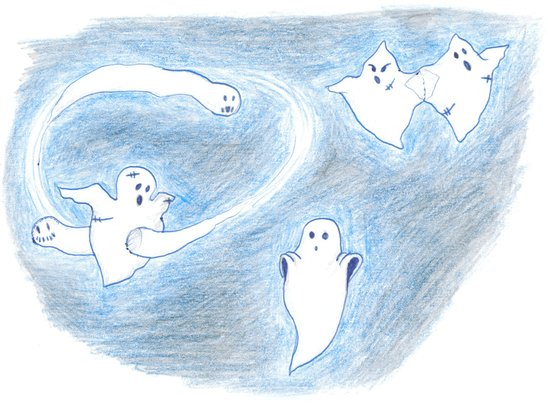
\includegraphics{phantoms}

  \centering\normalsize
  \textbf{\color{mypurpledark}Pointfreely embracing
  \textcolor{mypurplepurple}{infinite sequences} as useful fictions}

  \tiny

  \centering
  7th Workshop on Formal Topology in Venice \\
  April 16th, 2026

  \tiny

  Ingo Blechschmidt \\
  University of Antwerp

  \bigskip
  partially joint work with

  
\includegraphics[height=7em]{gabriele-buriola}\qquad
  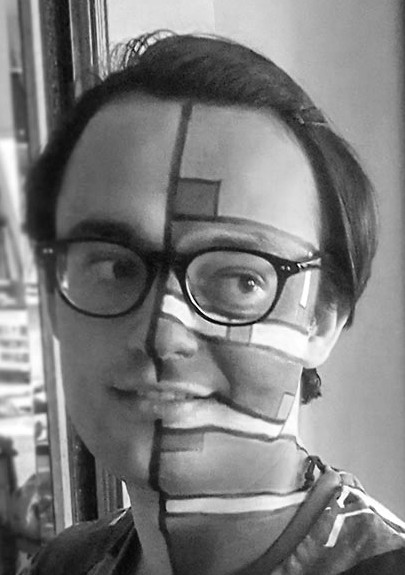
\includegraphics[height=7em]{alexander-oldenziel}\qquad
  
\includegraphics[height=7em]{jacopo-piccione}\qquad
  
\includegraphics[height=7em]{peter-schuster}

  Gabriele Buriola \textbullet{}
  Alexander Oldenziel \textbullet{}
  Jacopo Piccione \textbullet{}
  Peter Schuster
\end{frame}

\definecolor{mypurple}{RGB}{150,0,255}
\setbeamercolor{structure}{fg=mypurple}

\newcommand{\qmark}{
\includegraphics[height=0.7em]{question-mark}}
\newcommand{\qswitch}[3]{\only<1-#1>{\qmark}\only<#2->{#3}}
\newcommand{\ccmark}{\good{\cmark}}
\newcommand{\cxmark}{\bad{\xmark}}

\begin{frame}{What is a function in constructive mathematics?}
  \small
  \centering
  Function types are \bad{brittle}.

  \renewcommand{\arraystretch}{1.05}
  \begin{tabular}{@{\!\!\!\!\!\!}l@{\,}l@{\,\,\,}l@{\,\,}l@{\,\,}ll@{}}
    \toprule
    & statement & class. & neutr. & in $\mathrm{Eff}$ \\\midrule
    \normalnumber{0} & Every function is computable. & \cxmark & \qmark & \ccmark \\
    \normalnumber{1} & Every function has a zero or not. & \ccmark & \qmark & \cxmark \\
    \normalnumber{2} & Every path leaves the Kleene tree. & \cxmark & \qmark & \ccmark \\
    \normalnumber{3} & There is no surjection $\NN \twoheadrightarrow \RR$. &
    \ccmark & \qmark & \ccmark & False in parametrized realizability. \\
    \\
    \multicolumn{6}{c}{With \bad{adverse effects} throughout mathematics:} \\[0.1em]
    \normalnumber{4} & Dickson's lemma. & \ccmark & \qmark & \cxmark \\
    \normalnumber{5} & Products of streamless sets are streamless. & \ccmark & \qmark & \cxmark \\
    \normalnumber{6} & Products of wf.\@ relations is wf. & \ccmark & \qmark \\
    \normalnumber{7} & Every real is positive or not. & \ccmark & \qmark & \cxmark \\
    \normalnumber{8} & Every field has an algebraic closure. & \ccmark & \qmark & \cxmark & Implies a form of choice. \\
    \normalnumber{9} & Hilbert's basis theorem. & \ccmark & \qmark && {``If $A$ is Noetherian, so is $A[X]$.''} \\
    \normalnumber{10} & Locally Noetherian implies Noetherian. & \ccmark & \qmark &&
    {``If all $A[f_i^{-1}]$ are Noetherian, so is $A$.''} \\
    \normalnumber{11} & Krull's lemma. & \ccmark & \qmark &&
    {``If $x \in \bigcap_\mathfrak{p} \mathfrak{p}$, then $x$ is nilpotent.''} \\
    \normalnumber{12} & Fundamental theorem of Galois theory. & \ccmark & \qmark &&
    {``If $x \in L^{\mathrm{Aut}_K(L)}$, then~$x \in K$.''}
  \end{tabular}
\end{frame}

\begin{frame}{Harnessing formal topology}
  Let~$X$ be a set.

  Irrespective of \bad{function types}, there is a \good{robust} \hil{formal
  space}$^\star$~$X^\NN$ with \hil{basic opens}
  \[ \begin{array}{@{}c@{}}
    [x_0,\ldots,x_{n-1}] \\[0.3em]
  \text{\footnotesize pictured as the open ``$\{ f : \NN \to X \,|\, f(0) = x_0, \ldots,
  f(n-1) = x_{n-1} \}$''}
  \end{array} \]
  and \hil{coverings} \good{inductively generated} by
  \[
    [x_0,\ldots,x_{n-1}] \lhd \{ [x_0,\ldots,x_{n-1},a] \,|\, a \in X \}.
  \]
  \visible<2->{We can then explore:}

  \small

  \centering

  \visible<2->{\begin{tabular}{@{}r@{$\quad\xleftrightarrow{\quad1:1\quad}\quad$}l@{}}
    (absolute) points of $X^\NN$ & functions $\NN \to X$ \\
    \visible<3->{$E$-valued points of $X^\NN$ & morphisms $E \to X^\NN$ of spaces} \\
    \visible<4->{the generic point of $X^\NN$ & the identity morphism $X^\NN \to X^\NN$}
  \end{tabular}}

  \normalsize

  \visible<5->{\fmini{0.8\textwidth}{
    Guiding principle:
    Refer to \hil{all} points, not just the \bad{absolute points}.
  }}

  \raggedright
  \vfill
  \bigskip
  \scriptsize
  $^\star$ distributive lattice, site, locale, topos, arithmetic universe, \ldots
\end{frame}

\begin{frame}{Dialogues with oracles}
  For a predicate~$P$ on~$\mathrm{List}(X)$, we inductively define $P \mid
  \sigma$ (``$P$ bars the list $\sigma$'') by the following two clauses.
  \begin{enumerate}
    \item ``now'': If $P\,\sigma$, then~$P \mid \sigma$.
    \item ``later'': If~$P \mid \sigma a$ for all $a \in X$, then~$P \mid \sigma$.
  \end{enumerate}
  The assertion $P \mid \sigma$ expresses in a positive
  way that \hil{no matter how} the finite approximation~$\sigma$ evolves over time to
  a \hil{better approximation}~$\tau$, \hil{eventually}~$P\,\tau$ will hold.

  A witness of $P \mid \sigma$ is a \hil{dialogue tree} recording \hil{queries}
  to an oracle of type $\NN \to X$, eventually culminating with witnesses
  of~$P$ at the leaves.
  \pause

  \begin{columns}
    \begin{column}{0.48\textwidth}
      \begin{block}{A brittle definition}
        A set~$X$ is \bad{streamless} iff \\
        for every function~$f : \NN \to X$, \\
        there are numbers~$i < j$
        such that~$f(i) = f(j)$.
      \end{block}
    \end{column}

    \begin{column}{0.48\textwidth}
      \begin{block}{A robust definition}
        A set~$X$ is \good{Noetherian} iff
        $\mathrm{R} \mid [\,]$, \\
        where $\mathrm{R}\,[x_0,\ldots,x_{n-1}]$ iff \\
        there are numbers~$i < j$ such that~$x_i = x_j$.
      \end{block}

      \pause
      Equivalently: $\Box(\text{$X$ is streamless})$.
    \end{column}
  \end{columns}
\end{frame}

\begin{frame}{Elephant functions}
  \textbf{Def.} An \hil{elephant function} from~$X$ to~$Y$ is a \hil{coherent
  family} of~$E$-points of the space~$Y^X$, one for each space~$E$, i.\@e. a
  family consisting of
  \begin{itemize}
    \item for each space~$E$, a morphism~$f_E : E \to Y^X$,
  \end{itemize}
  such that
  \vspace*{-2em}
  \begin{itemize}
    \item for each morphism~$g : F \to E$, the diagram
    $
      \vcenter{\xymatrix@R=0.5em{
        E \ar@/^/[rrd]^{f_E} \\
        && Y^X \\
        F \ar@/_/[rru]_{f_F} \ar[uu]^g
      }}
    $
    commutes.
  \end{itemize}
  \bigskip

  \begin{columns}
    \begin{column}{0.5\textwidth}
      \textbf{Prop.} For a function~$f : (\NN \to \mathbbm{2}) \to \NN$, TFAE:
      \begin{enumerate}
        \item $f$ can be extended to an elephant function from~$\mathbbm{2}^\NN$
        to~$\NN$.
        \item $f$ is uniformly continuous.
        \item $f$ is eloquent (i.\@e. given by a dialogue).
      \end{enumerate}
    \end{column}

    \begin{column}{0.5\textwidth}
      \textbf{Prop.} For a function~$f : [0,1] \to \RR$, TFAE:
      \begin{enumerate}
        \item $f$ can be extended to an elephant function from~$[0,1]$ to~$\RR$.
        \item $f$ is uniformly continuous.
        \item $f$ is eloquent (in a suitable real-number-oracle querying sense).
      \end{enumerate}
    \end{column}
  \end{columns}
\end{frame}

\begin{frame}{Modal language for embracing points}
  \textbf{Def.} A statement~$\varphi$ holds \ldots
  \vspace*{-0.3em}
  \begin{itemize}
    \small
    \item \hil{everywhere} \tabto{2.15cm}($\necessary\varphi$)\tabto{3.08cm}
    iff it holds \hil{over every space}
    (over the current base).
    \item \hil{somewhere} \tabto{2.15cm}($\possible\varphi$)\tabto{3.08cm} iff
    it holds \hil{over some positive space}.
    \item \hil{proximally} \tabto{2.15cm}($\xpossible\varphi$)\tabto{3.08cm}
    iff it holds \hil{over some positive overt space}.
  \end{itemize}
\end{frame}

\end{document}
